%%%%%%%%%%%%%%%%%%%%%%%%%%%%%%%%%%%%%%%%%
% Journal Article
% LaTeX Template
% Version 1.3 (9/9/13)
%
% This template has been downloaded from:
% http://www.LaTeXTemplates.com
%
% Original author:
% Frits Wenneker (http://www.howtotex.com)
%
% License:
% CC BY-NC-SA 3.0 (http://creativecommons.org/licenses/by-nc-sa/3.0/)
%
%%%%%%%%%%%%%%%%%%%%%%%%%%%%%%%%%%%%%%%%%

%----------------------------------------------------------------------------------------
%	PACKAGES AND OTHER DOCUMENT CONFIGURATIONS
%----------------------------------------------------------------------------------------

\documentclass[twoside]{article}

\usepackage{graphicx} % Package to display images

\usepackage[sc]{mathpazo} % Use the Palatino font
\usepackage[T1]{fontenc} % Use 8-bit encoding that has 256 glyphs
\linespread{1.05} % Line spacing - Palatino needs more space between lines
\usepackage{microtype} % Slightly tweak font spacing for aesthetics

\usepackage[hmarginratio=1:1,top=32mm,columnsep=20pt]{geometry} % Document margins
\usepackage{multicol} % Used for the two-column layout of the document
\usepackage[hang, small,labelfont=bf,up,textfont=it,up]{caption} % Custom captions under/above floats in tables or figures
\usepackage{booktabs} % Horizontal rules in tables
\usepackage{float} % Required for tables and figures in the multi-column environment - they need to be placed in specific locations with the [H] (e.g. \begin{table}[H])
\usepackage{hyperref} % For hyperlinks in the PDF

\usepackage{lettrine} % The lettrine is the first enlarged letter at the beginning of the text
\usepackage{paralist} % Used for the compactitem environment which makes bullet points with less space between them

\usepackage{abstract} % Allows abstract customization
\renewcommand{\abstractnamefont}{\normalfont\bfseries} % Set the "Abstract" text to bold
\renewcommand{\abstracttextfont}{\normalfont\small\itshape} % Set the abstract itself to small italic text

\usepackage{titlesec} % Allows customization of titles
\renewcommand\thesection{\Roman{section}} % Roman numerals for the sections
\renewcommand\thesubsection{\Roman{subsection}} % Roman numerals for subsections
\titleformat{\section}[block]{\large\scshape\centering}{\thesection.}{1em}{} % Change the look of the section titles
\titleformat{\subsection}[block]{\large}{\thesubsection.}{1em}{} % Change the look of the section titles

%----------------------------------------------------------------------------------------
%	TITLE SECTION
%----------------------------------------------------------------------------------------

\title{\vspace{-25mm}\fontsize{24pt}{10pt}\selectfont\textbf{Major League Hacking: Hackathon Communities}} % Article title

\date{December 2013}

\author{
\large
\textsc{Arda Aysu}\\
\normalsize{Rutgers University}\\
\normalsize{ardaaysu@hotmail.com}
\and
\large
\textsc{Billy Lynch}\\
\normalsize{Rutgers University}\\
\normalsize{wlynch92@gmail.com}
\and
\large
\textsc{Alex Tang}\\
\normalsize{Rutgers University}\\
\normalsize{alex.m.tang@gmail.com}
\vspace{-5mm}
%\large
%\textsc{John Smith}\thanks{A thank you or further information}\\[2mm] % Your name
%\normalsize University of California \\ % Your institution
%\normalsize \href{mailto:john@smith.com}{john@smith.com} % Your email address
%\vspace{-5mm}
}

%----------------------------------------------------------------------------------------

\begin{document}

\maketitle % Insert title

%\thispagestyle{fancy} % All pages have headers and footers

%----------------------------------------------------------------------------------------
%	ABSTRACT
%----------------------------------------------------------------------------------------

%\begin{abstract}

%\noindent \lipsum[1] % Dummy abstract text

%\end{abstract}

%----------------------------------------------------------------------------------------
%	ARTICLE CONTENTS
%----------------------------------------------------------------------------------------

\begin{multicols}{2} % Two-column layout throughout the main article text

\section{Introduction}
Major League Hacking (MLH) refers to the series of hackathons, which are events where
software engineers and computer scientists collaborate and compete with other groups. 
Hackathons are held worldwide, and many of them at well-known universities. By looking 
at hackathon attendance we are able to create a weighted directed multigraph showing the 
activity of each school. The data provided, while small, can be used to show how 
often schools interact with each other in the hacking	community and the optimal 
locations for new hackathons to promote the growth of the MLH scene.

%------------------------------------------------

\section{Graph Representation}

Each vertex represents a school that has attended or hosted a hackathon. The directed
edges represent the number of attendees that went from each school to a hackathon 
held at another school. Since there was only data for five hackathons available 
(RU, NYU, MIT, UMich, UPenn), all other schools will have an in-degree of zero.


\begin{figure}[H]
\caption{Undirected MLH Graph}
\centering
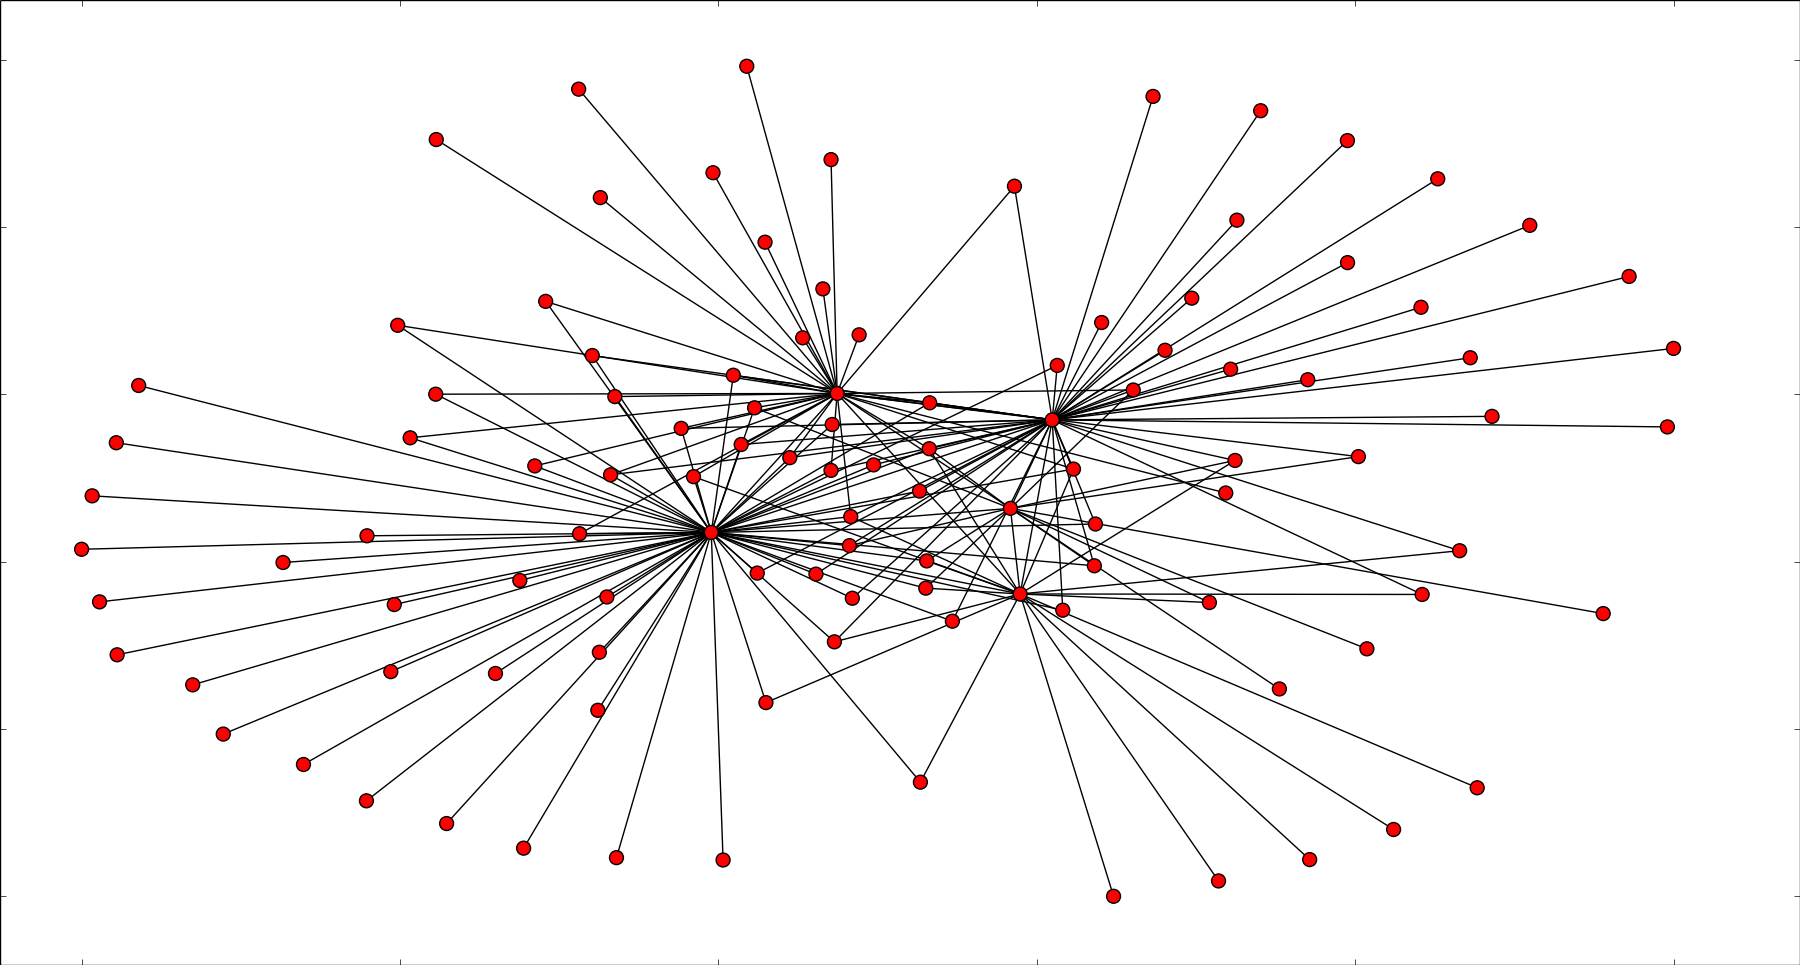
\includegraphics[width=\linewidth, trim = 1cm 1cm 1cm 1cm, clip]{mlh_graph.png}
\end{figure}

%\begin{compactitem}
%\item Donec dolor arcu, rutrum id molestie in, viverra sed diam
%\end{compactitem}

%------------------------------------------------

\section{Implementation}
A python module was made using CSV data from MLH and several external Python 
libraries:
\begin{compactitem}
\item NetworkX: A graph manipulation library
\item matplotlib: A graph visualization library\\
\end{compactitem}

A map based graph visualization was made by using D3.js and parsed csv data.\\

Users can view different properties of the graph by using the functions and dictionaries
provided in mlh\_graph. Once mlh\_graph.py parses the graph from the csv file, you can 
then use NetworkX to write your own scripts to manipulate the graph. See draw\_cliques.py
for an example.
%------------------------------------------------

\section{Algoithms and Complexity}

\subsection{Max Outdegree}
This routine simply iterates through the list of nodes in the graph once and 
determines which vertex has the largest degree of outgoing verticies. This 
algorithm runs in O(n) time, where n is the number of vertices in the graph.

\subsection{Max Indegree}
An analogous process to Max Outdegree, therefore O(n).

\subsection{Clique}
This algorithm finds complete subgraphs in a given graph. In particular, we
are interested in finding the largest clique in the graph. This algorithm is
NP Complete.

\subsection{k-clique Communities}
Also known as the Clique Percolation Method, this algorithm finds "communities"
of cliques, or adjacent cliques of size > k vertices that share k-1 vertices.

\begin{figure}[H]
\caption{Example k-clique community}
\centering
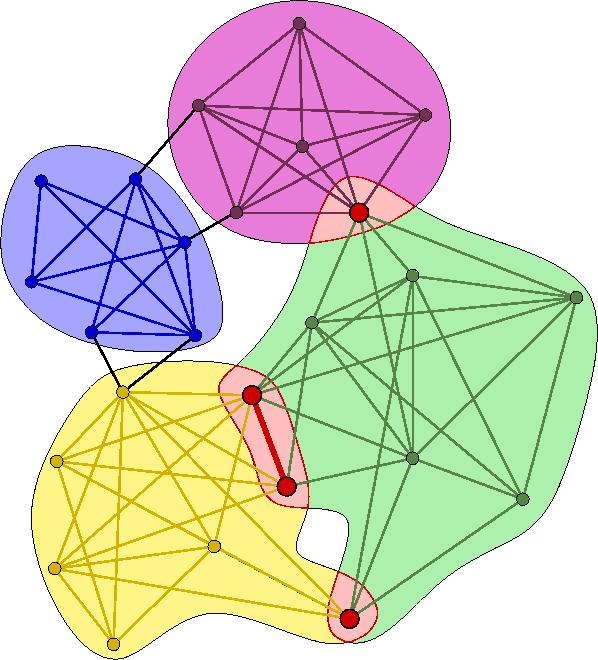
\includegraphics[width=.5\linewidth]{communities_example.jpg}
\end{figure}

%------------------------------------------------

\section{Results}
The University of Maryland was found to have the highest out-degree, and thus
the highest overall attendance and presence in the observed MLH community. This
suggests that since the university did not yet host a hackathon, they would be
an optimal site for an event that would generate high attendance. \\\\
With more data we would be able to look at cliques of schools to determine which 
schools interact with each other the most, and then use this information to suggest 
and identify possible new partnerships. However, with our limited data set it is
more informative to look at the largest k-clique community. A k-clique community
is defined as the maximal union of k-cliques that can be reached from each other
through a series of adjacent k-cliques, and two k-cliques are considered to be
adjacent if they share k-1 nodes. To observe cliques, undirected graphs were
used so as to prevent excluding schools which had not yet hosted a hackathon.
Reflexive loops also exist to denote attendees that go to the school which
hosted the hackathon. \\\\

\begin{figure}[H]
\caption{MLH 5-clique Community}
\centering
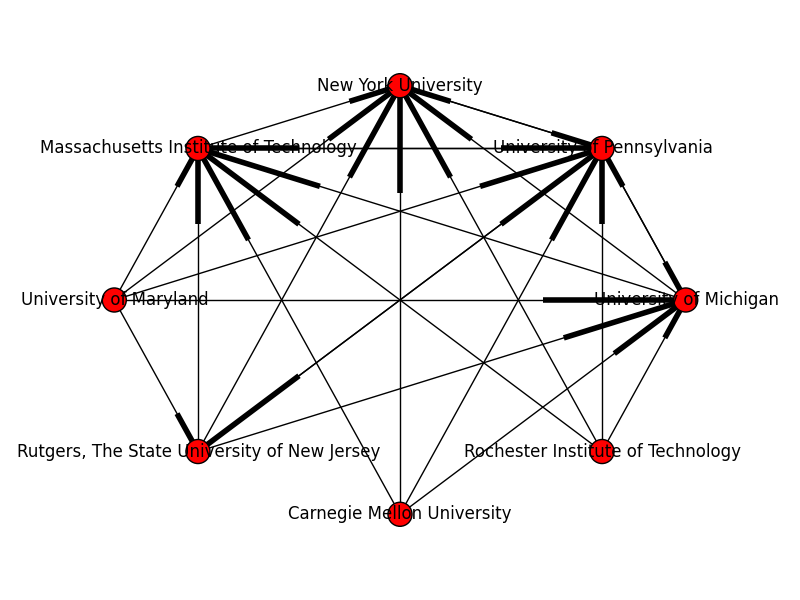
\includegraphics[width=\linewidth, trim = 1cm 1cm 1cm 1cm, clip]{mlh_community.png}
\end{figure}

By analyzing the data provided from the five hackathons, it was found that the 
University of Maryland (UMD), Rutgers University (RU), University of Pennsylvania 
(UPenn), New York University (NYU), University of Michigan (UMich), Rochester 
Institute of Technology(RIT), Carnegie Mellon University (CMU), and Massachusetts
Institute of Technology (MIT) are in a 5-clique community. This suggests that
hackathons hosted at schools in the clique community which do not already host
hackathons would receive good attendance from the other schools mentioned and
further strengthen the regional MLH community. RIT appears to be an outlier in 
this data set due to its low attendance, so it is beneficial to set some minimum
threshold (such as having a outdegree above the mean of all schools) to be considered.
Combined with the fact that UMD and CMU have substancial attendance at other hackathons, 
this graph suggests that a hackathon held there would be the most beneficial for 
both growing and reinforcing the MLH community.

%------------------------------------------------

\section{Conclusion}

By looking at data for hackathon attendance, it was found that a 5-clique 
community exists between UMD, RU, UPenn, NYU, UMich, RIT, CMU, and MIT.
Seeing how UMD and CMU do not currently host their own hackathon and contributes a
substancial number of students to make them active members in the community, it is 
suggested that this would be an optimal site for the MLH community to add another
hackathon.

%----------------------------------------------------------------------------------------
%	REFERENCE LIST
%----------------------------------------------------------------------------------------

\begin{thebibliography}{99} % Bibliography - this is intentionally simple in this template

\bibitem{Palla}
Gergely Palla, Imre Derenyi, Illes Farkas, and Tamas Vicsek (2005).
\newblock Uncovering the overlapping community structure of complex networks in nature and society Nature 
\newblock doi:10.1038/nature03607

\end{thebibliography}

%----------------------------------------------------------------------------------------

\end{multicols}

\end{document}
